\chapter{Introduction}
\label{chp:INTRO}


%%%%%%%%%%%%%%%%%%%%%%%%%%%%%%%%%%%%%%%%%%%%%%%%%%%%%%%%%%%%%%%%%%%%%%%
\section{P2P MMVEs}
\label{background}

Peer-to-Peer (P2P) Massively Multiplayer Online Games (MMOGs) have received significant attention from the research community, since
the first publication on the subject by Knutssonn et al. in 2004 \cite{knutsson_p2p_first}. P2P MMOGs promise to solve many issues prevalent in
today's Client/Server (C/S) based MMOGs. Some key issues have to be solved before P2P MMOGs can be implemented commercially. Over the past few years,
researchers have been addressing these challenges.

The focus of this paper is exclusively on one of the key challenges present in P2P MMOGs, namely: state persistency. The implementation of state
persistency in P2P MMOGs allows for the storage of game data. The fact that game data must now be distributed amongst various peers in the network
creates challenges not usually present in classic C/S MMOGs.

The paper classifies the techniques used in documented P2P MMOG architectures and discusses the advantages and disadvantages of the different types
of storage. The paper also shows that no current storage type is well suited to P2P MMOGs. As the field of P2P MMOGs is a growing one, it is believed
that a comprehensive survey of persistency techniques is required to act as a basis for further research into the field.

To the best of our knowledge, such a classification, where a focus is placed specifically on state persistency in P2P MMOGs, has not been undertaken
in the literature. Other surveys, relating to P2P MMOGs and P2P overlays in general are discussed in Section \ref{related_work}. For each included
survey, the differences between this paper and the included survey are discussed.

The remainder of this paper is structured as follows: the field of P2P MMOGs is introduced in Section \ref{p2p_network_architectures}, which contains
an introduction to P2P overlays, the major advantages of P2P MMOGs and the key challenges that P2P MMOGs face. An introduction to some classic
consistency models, currently used in computer games, are introduced in Section \ref{classic_models}. Section \ref{related_work} discusses some
related surveys that have been completed in the field of P2P MMOGs and P2P applications in general. Section \ref{p2p_mmog_state_persistency} contains
an analysis of different types of distributed storage for MMOGs. The section defines characteristics against which all storage schemes are evaluated.
The section concludes with recommendations to implementers as to the applicability of the different types of storage to different types of games.
Section \ref{conclusion} concludes the paper by providing a brief summary and suggesting a number of areas for future work.

\section{Peer-to-Peer MMOG network architectures}
\label{p2p_network_architectures}

In 2004, an architecture using the peer-to-peer networking model to host MMOGs was proposed by Knutsson et al. \cite{knutsson_p2p_first}. This
revealed a new research field, which attempts to establish the P2P model as a viable alternative to the classic C/S and Client/MultiServer (C/MS)
architectures. This architecture does, however, still have a few major issues that need to be solved before MMOGs can be developed that use it. If
these issues, discussed in Section \ref{key_challenges}, can be solved, a P2P architecture holds some powerful advantages over a C/S system.

The core idea of the P2P model is that each peer contributes sufficient resources to the network to host itself. This also means that all functions
of the server in the classic C/S model are distributed amongst all peers. There are many areas where the P2P model can improve on the classic C/S
model. These areas are robustness, scalability, provider cost, latency, server bandwidth and handling of peak transient load.

\subsection{Structured and unstructured P2P overlay networks}
\label{overlays}

P2P networks are created and maintained in the application layer of the Open Systems Interconnection (OSI) model protocol stack. This application
layer network is called the P2P overlay. Peers in an overlay network might have neighbours that have no relationship to their physical position in
the underlying network. Overlays can broadly be classified into structured and unstructured types. The classification is mostly based on the
differing methods of routing and content retrieval in the network. This section only provides a brief comparison between structured and unstructured
overlays. For a detailed comparison between the two types that also deals with many of the myths of structured overlays, please refer to
\cite{Castro_structured_overlay_myths}.

With unstructured approaches, one is never assured that a data item will be retrieved, even if that data item is present in the network. If many
duplicates of a data item are contained in the network, this becomes less of a problem, since it is assumed that the request will be routed to some
set of nodes that do  possess the item.

An unstructured architecture works well for content sharing and Voice over Internet Protocol (VoIP) networks, for example: P2P TV, BitTorrent,
Gnutella and Skype. The reason for this is the high level of duplication in these networks, especially for popular content. It is also easier to
perform keyword searches in unstructured networks and the overlay requires less maintenance.

Because there is no assurance that a data item might be retrieved from an unstructured network, especially when that item is scarce, unstructured
overlays are not considered adequate as a basis for P2P MMOGs, where all data items must be available at all times.

Structured overlays have been proposed that provide for efficient routing and reliable retrieval of data items. Some of these well known overlays
are: CAN \cite{CAN}, Chord \cite{chord}, Tapestry \cite{tapestry} and Pastry \cite{pastry}.

The basic idea of a structured overlay is that all nodes are identified by unique identifiers (IDs). A popular method to create the IDs is to use
hashes to a circular key space. Any node in the overlay network is then able to efficiently route a query with a given ID, to a node with an ID
closest to the given ID. An accurate comparison is that unstructured overlays are good at finding ``hay'', while structured overlays are good at
finding ``needles'' \cite{Rodrigues_acm_comms_p2p}.

%TODO: Add something about the effect of the hashing and why it's important

\subsection{Advantages}
\label{p2p_advantages}

There are various advantages to moving from C/S to P2P in MMOGs. These include: increased robustness, improved scalability, lower operator costs,
improved handling of transient player load and lower latencies.

The P2P system is robust, because there is no server that can fail, only individual peers. Individual peers failing will not affect any other peers
other than the peer that failed. This behaviour makes game down-time extremely unlikely.

Furthermore, because every peer hosts itself, the system is scalable. Another advantage is that no extra costs are incurred from an operator
perspective, when more peers join the network. This will also allow for efficient handling of transient loads. If many players suddenly enter the
game no resource provisioning issues will arise, since peers already possess their required resources.

P2P architectures also create a lot of opportunity for independent developers, because a large initial investment is no longer required to purchase
the expensive server hardware. Not only are hardware costs reduced, but running costs are also reduced. The bandwidth required by the game server is
now shared amongst users, which means that very little bandwidth costs will be incurred by the provider.

Latency is also improved, because it is now possible to directly communicate between peers and it is not necessary to communicate via a server. There
is also no single server that has to process game events. Game events need only be processed by other peers who find the specific events of interest.
The distribution of the load as well as direct communication will further reduce latency. Game events are defined in Section \ref{terminology}.

\subsection{Key challenges}
\label{key_challenges}

%State persistency, compared to state consistency
A key challenge with any networked game is how to maintain state consistency between root and replica objects. A root object is the authoritive
version of an object and the replica object is usually a local non-authoritive version. Root objects are usually found on the server and replica
objects are found in the local object cache of clients. The method by which the states between root and replica objects are updated is called the
consistency model. Solving the state consistency problem for P2P MMOGs is one of the major development challenges.

A recent article has identified six key challenges of P2P systems: Interest Management, Game Event Dissemination, Non-player Character (NPC) Host
Allocation, Game State Persistency, Cheating Mitigation and Incentive Mechanisms \cite{Fan_deisgn_issues_p2p}. A brief overview of these challenges
will be introduced below.

\begin{figure}[htbp]
 \centering
 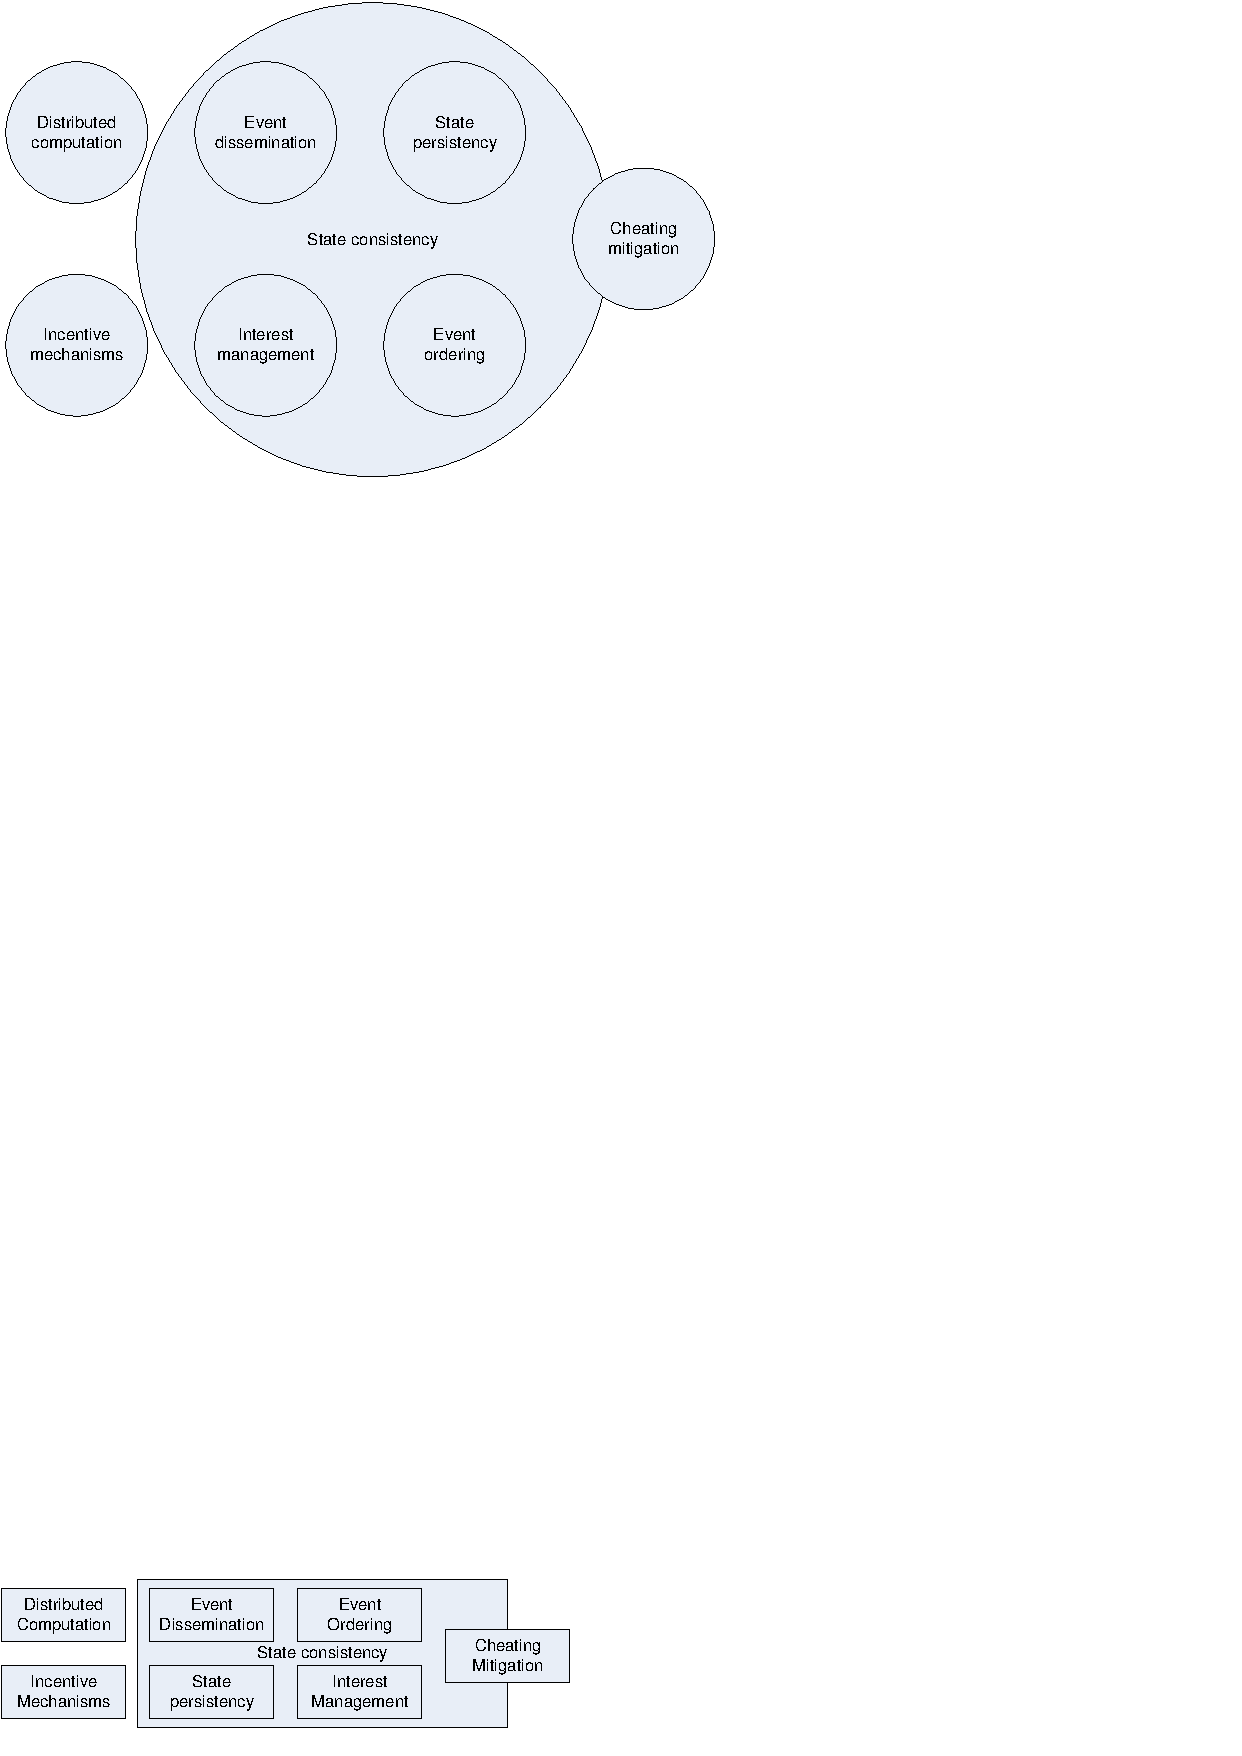
\includegraphics[clip=true, viewport=0cm 0cm 10cm 3cm, width=0.5\columnwidth]{Component_VEN}
 \caption{VEN diagram showing the relationship between different characteristics}
 \label{fig_component_ven}
\end{figure}
%
As shown in Figure \ref{fig_component_ven}, of the six challenges mentioned, Interest Management, Game Event Dissemination and Game State Persistency
all form part of State Consistency, with some aspects of Cheating Mitigation also a part of State Consistency. Also part of state consistency is
event ordering, which deals with how to ensure that the system remains causal \cite{GauthierDickey_low_latency_event_ordering}.

Another challenge for P2P systems is the required peer bandwidth. In a paper by Miller and Crowcroft, a packet simulator was created to determine the
required bandwidth and effective latency, if a game such as World of Warcraft were to be implemented using P2P technologies
\cite{Miller_p2p_infeasability}. Their simulation results indicate that today's networks are not able to host P2P MMOGs, with the required bandwidth
and latency constraints. Such a significant result requires verification, but at the least, it shows that reducing bandwidth and latencies for P2P
MMOGs should be a primary design requirement.

It should be noted that the overview presented here is only an overview of the different techniques and general trends present in the different areas
of peer-to-peer MMOGs. This overview does not presume to present an exhaustive list of papers in these areas, rather to place the topic of state
persistency in context; to show readers how state persistency fits into the context of peer-to-peer games and to allow readers to distinguish
between, for example, the topics of state persistency, interest management and event dissemination.

%Describe key challenges
\subsubsection{Interest management}
\label{key_challenges_im}

Interest management is used to determine the smallest amount of information that a peer requires, in order to present an accurate representation of
the world to players. In consistency terms, it provides a means to determine which replica objects require updates of the root object. The idea is
not specific to P2P MMOGs and was already formally suggested in \cite{First_IM} and later with greater focus on a distributed environment in
\cite{Whang_agent_based_IM}. Extensive research has been done into solving AoI problems and a comparison of techniques can be found in
\cite{Boulanger_IM_compare} and \cite{IM_and_ED_survey_Krause}.

The main idea is that a player has a limited visual range and area around the player in which it can interact with objects. The player requires
update information of all objects in this area, called the player's Area of Interest (AoI). AoI calculations also rely on the fact the a player's
direction and velocity of movement cannot change instantaneously and are bounded in magnitude.

\subsubsection{Event dissemination}

Event dissemination deals with how information is sent to peers after interest management determines which information should be sent. In consistency
terms, it determined how events and updates are distributed in the network. The first application of event dissemination for online games can be
found in \cite{first_GED}. Recently, ALM and unicast techniques of event dissemination have become popular, depending on the grain of the event
dissemination. ALM is used, instead of router level multicast, because of a lack of general support for this technology at the router level
\cite{ip_multicast_deployment_issues}.

\subsubsection{Cheating mitigation}
\label{key_challenges_cheating}

Cheating mitigation has been identified as a major issue for P2P systems \cite{knutsson_p2p_first}, \cite{challenges_p2p_gaming},
\cite{cheat_proof_event_ordering}. The challenges reside in the fact that peers are not under the control of the game producer. Since all server data
are distributed amongst peers, all peers have access to sections of the server data. Peers also have access to the distributed server code. One
advantage that can be exploited to prevent cheating is that no peer contains all server data and no single peer has more authority than another.

There are various security issues that are usually classified according to the level in the protocol stack where they occur. The areas identified by
\cite{cheat_proof_event_ordering} and expanded upon by \cite{cheating_taxonomy} are: game level, application level, protocol level and infrastructure
level. This is consistent with the generally used layered security model \cite{distributed_systems_security}.

As with all taxonomies, all cheats may not cleanly fit into one if these boxes, some cheats may occur over multiple levels or a cheat with a specific
outcome can be implemented differently on different levels. The field of P2P security has recently received more attention than in the past and has
started to bear fruit \cite{survey_p2p_game_cheats}. This is, however, an ongoing research field with many issues still open. For an in-depth review
of the security issues facing peer-to-peer system in general, refer to \cite{p2p_security_issues}. These issues are the same issues facing P2P MMOGs,
with the exception of the game and application layer issues.

\subsubsection{Incentive mechanisms}

P2P schemes require all players to share resources in order to ensure correct functionality. The issue with this is that players might not want to
share their resources, but still benefit from the resources of others. This is where incentive mechanisms become important. The function of these
mechanisms is to ensure that all players contribute resources, by incentivised contribution.

All distributed resource sharing models require incentive mechanisms. For example, Bittorrent systems use the tit-for-tat protocol to ensure that all
people downloading data are also contributing data \cite{tit_for_tat}. Such mechanisms are also required with P2P MMOGs. One advantage in designing
an incentive algorithm for a P2P MMOG is that players can be made to contribute resources for the duration of play. The issues with file sharing
systems are not present where a peer, after downloading a file, has no more incentive to contribute. When a peer plays a game, incentive can be
created to provide resources for the duration of the game.

\subsubsection{Distributed computation}

Non-Player Characters (NPCs) are characters that are not controlled by any human player, but are rather controlled by some artificial intelligence
routine or script executing on some host machine. These characters represent the traders and monsters in MMOGs and usually contain sets of rules that
determine how they should interact with Player Characters (PCs) as well as their own state information. An NPC's state can be how much money and
items it has to trade or how much health it still has after being attacked by a player.

In the original NPC host allocation classification by Fan, both NPC state and computational routines are combined into a single category
\cite{Fan_phd}. In the classification presented below, NPC state forms part of normal game state persistency, since NPC objects are game objects like
any other. The NPC routines requiring computational power are grouped under the heading of distributed computation. This heading is meant to include
the distribution of all in game computational elements.

Some game objects require computational power to function. An example of this is the Artificial Intelligence routines of NPCs or the computation of
physics effects on in-game objects. Some architectures assume that the computational requirements will be fulfilled where the object state is hosted
\cite{solipsis}, but other schemes exist that allow for the CPU power to be distributed amongst peers. One such scheme makes use of a ``job board''
like mechanism, where tasks are advertised on specialised super peers. Other peers monitor these super peers and may elect to perform the advertised
tasks \cite{fan_mediator_paper}.

\subsubsection{Game state persistency}

Game state persistency involves the storage of game objects, either in primary or secondary storage. In a recently completed PhD on the subject of
P2P MMOGs, Lu Fan had this to say about state persistency: ``Game state persistency is a major challenge for P2P MMOGs as existing P2P storage
infrastructures are designed to support file sharing, and seldom fulfil the performance and security requirements of a MMOG. \ldots the persistency
area is still immature with many problems waiting to be investigated.'' \cite{Fan_phd}.

State persistency is treated as a sub domain of state consistency, in that state persistency models define where and how the root or authoritive
objects are stored. It is assumed that replica objects are always stored in the primary memory of the clients that immediately require the
information contained in the root object.

The issue of game state persistency in P2P MMOGs is the focus of this paper and the remainder of the paper will deal exclusively with this subject.
However, before the different storage types are reviewed, some classic C/S models are presented for comparison with the fully distributed model.

\section{Related work}
\label{related_work}

In this section we discuss related surveys on P2P MMOGs. This will set the context for the discussion on state persistency for P2P MMOGs.

In 2007 Schiele et al. published the paper: ``Requirements of Peer-to-Peer-based Massively Multiplayer Online Gaming''
\cite{Schiele_p2p_requirements}. This paper presents a broad overview of some key requirements that P2P MMOGs should possess, to function correctly
under any load for any period of time. These are: distribution, consistency, self-organisation, persistency, availability, interactivity,
scalability, security, efficiency and maintainability. The focus of this paper is on the persistency requirement identified in the paper by Schiele.

In 2005, Hasan et al. published the manuscript: ``A Survey of Peer-to-Peer Storage Techniques for Distributed File Systems''
\cite{Hasan_distributed_storage_survey}. The manuscript describes different techniques used to store data in a distributed fashion. The difference
between the paper by Hasan et al. and this paper is that this paper focusses on storing data for gaming applications, which have other requirements
than normal file storage. The contents of the paper by Hasan et al. is also encapsulated in the overlay storage section of this survey.

Krause presented ``A Case for Mutual Notification: A survey on P2P protocols for Massively Multiplayer Online Games.''
\cite{IM_and_ED_survey_Krause}. The protocols discussed in this survey focussed on the areas of interest management and event dissemination. Three
protocols were presented: ``Application Layer Multicast (ALM) based protocols'', ``Supernode based protocols'' and ``Mutual notification based
protocols''. The first two protocols deal with region-based interest management techniques that employ supernodes, also called super peers, and ALM
to achieve state consistency. The third protocol, which is presented as an alternative to region-based techniques, is a distance-based technique,
making use of Voronoi diagrams to achieve state consistency.

While the survey by Krause is also in the area of P2P MMOGs, it deals with the topics of interest management and event dissemination and not with the
topic of state persistency. In other words, it explains how updates to objects may be sent to earlier versions of an object, but not how these
objects may be stored.

Webb and Soh presented ``A Survey on Network Game Cheats and P2P Solutions'' \cite{survey_p2p_game_cheats}. The paper introduces a cheat
classification scheme, defining different ``levels'' of cheating, along with some examples of cheats in each level. For each example given, the
authors also discuss possible solutions to these cheats. The difference between this paper and the survey paper presented by Webb and Soh, is their
paper deals with securing the information stored in objects as well as securing updates made to objects, while this paper deals with storing those
objects.

%Amoretti's survey paper on P2P overlay schemes in general
The previously mentioned articles deal with other issues present in P2P MMOGs, namely interest management, event dissemination and security. The
paper by Amoretti: ``A Survey of Peer-to-Peer Overlay Schemes: Effectiveness, Efficiency and Security'', provides details of the broader area of P2P
overlay schemes \cite{amoretti_p2p_overlay_schemes_survey}. The paper focuses on security issues present in P2P overlay schemes, while also
introducing hybrid, unstructured and structured overlays and provides an extensive list of applications of the different schemes in different areas.

Three areas present in Amoretti's survey and also related to this survey are: ``Content sharing'', ``distributed storage'' and ``gaming''. The
content sharing technologies described in Amoretti's work are considered forms of overlay storage, further discussed in Section
\ref{overlay_storage}. While Amoretti's survey gives a broad description of P2P gaming in general and why it should be a viable alternative to a C/S
system, this survey deals specifically with the area of P2P MMOGs and more specifically, with state persistency in P2P MMOGs.

%Zhang's C/S persistency survey, describing when to perform which types of state updates.
%A paper recently published by Zhang et. al. deals with persistency in C/S MMORPGs \cite{zhang_cs_persistency_survey}. The paper investigates when
%game objects should be made persistent, i.e. written to secondary storage from primary storage. It distinguishes between data that should immediately
%be written to storage, such as an object changing hands in a trade, and data that only has to be written every other update, such as position
%updates. The paper then continues to define some schemes by which the number of position updates might be reduced as well as stating that MMOG
%persistence schemes are not widely published and are usually implementation specific.
%
%The paper by Zhang et. al. is related to this survey paper in that it looks at persistency and also provides information on what is required in a
%persistency scheme. The major difference between Zhang et. al.'s paper and this survey is that it deals with a C/S architecture and focusses on when
%to update objects, not where those objects will be stored.

\section{Objectives and contributions}
\label{objectives}


\section{Overview of this work}
\label{overview_intro}
